\documentclass[12pt]{report}
\usepackage{amsmath}
\usepackage{amssymb}
\usepackage{graphicx}
\usepackage{hyperref}
\usepackage{color}
\usepackage{float}
\begin{document}
		\title{Chromatin Architecture Post UVC damage- Summary of Results}	
		\author{Ofir Shukron}	
		\maketitle
		Here we present the main findings 
		\begin{itemize}
			\item Post UVC chromatin undergoes conformational changes such as unpacking straightening caused by repair mechanism proteins crowding and active force
			\item During this time both DNA and histones leave the ROi at the same proportion. 
			\item Repair mechanism further slides histones to exposes damage DNA. This causes additional loss of DNA and histone but in different proportions 
			\item During repair mechanism crowding, the damage zone, marked by the presence of repair mechanism, expands from about 1 $\mu  m$ to 1.7 $\mu m$
			\item We offer a prototypical 1D situation in which sliding and pushing causes loss in different proportions 
			\item We offer a formula to calculate the total expansion attributed to sliding 
			\item To estimate the contribution of pushing and sliding we analyze the data, based on preservation of material in the patch and fitting a polynomial to the gain function, we estimate the contribution of sliding and note that pushing is active continuously 			
			\item [not done yet] we validate our analysis method on UV dose dependent data
			\item To examine the organization of the  chromatin post repair, we perform simulations. We calibrate our simulation framework to 20\% loss of DNA after linkers have been removed by repair proteins, and volume of exclusion was placed around each damaged point. We slowly introduce cross-links to the levels they were before. 
			The measure of similarity is the mean number of neighbors each monomer in the ROi has relative to what it had previously
			
		\end{itemize}
		
		\section{Conceptual histone sliding model}
		   \begin{figure}
		   	\centering
		   	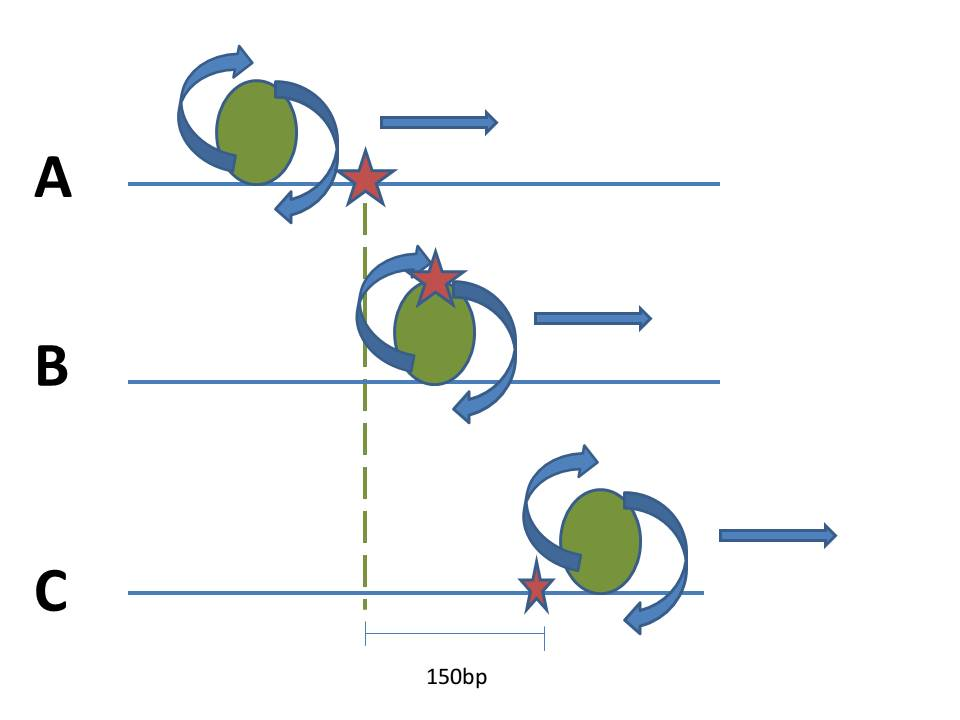
\includegraphics[width=0.7\linewidth]{Images/SlidingModel/histoneSlidingSingle}
		   	\caption{{Three time points during a displacement of damage site (red star) caused by histone rolling. The displacement of the damage site is equivalent to the length of DNA wrapped on a histone. A displacement is relative to some reference point, like the origin, and does not refer to an actual motion on the DNA}}
		   	\label{fig:histoneSlidingSingle}
		   \end{figure}
		   
		   \begin{figure}
		   	\centering
		   	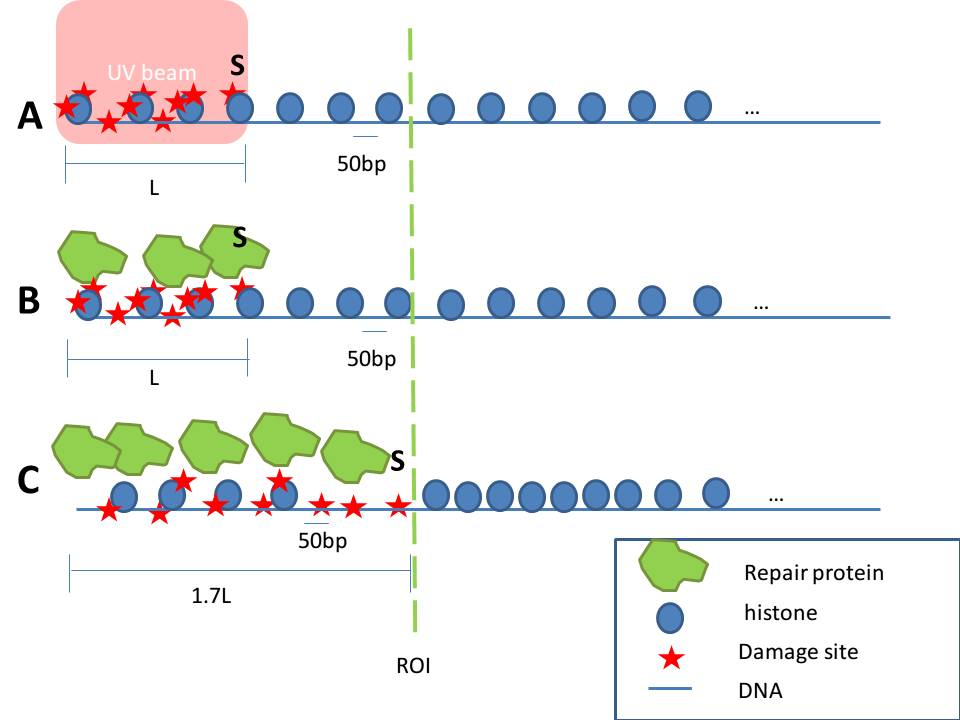
\includegraphics[width=0.7\linewidth]{Images/SlidingModel/histoneSlidingMulti}
		   	\caption{Expansion of the ROI due to nucleusome rolling. \textbf{A}. a UV beam (transparent red) damages DNA, with the point $S$ being the rightmost damage site \textbf{B}. Repair proteins (green polygons) are recruited to the damage site and start to expose the DNA in order the repair damages. \textbf{C}. Sliding the nucleosomes to the right in order to expose damage sites, translates the point $S$ to the right until $S$ reached $\sqrt{3}L$. Repair proteins are present at the new location. The presence of repair proteins in $\beta L$ indicates the ROI's boundary (vertical dashed green line). All DNA and histones to the right of $S$ are lost}
		   	\label{fig:histoneSlidingMulti}
		   \end{figure}
		   
		To explain the imbalance between the loss of histone and DNA we put forward a 1D histone sliding model. Histones and DNa are lost from the ROi by two mechanisms, one of pushing the DNa caused by repair mechanism crowding, and the second by sliding histones. We note that by histone sliding, the pushing of DNA is present but not conversely.
		DNA loss fraction
		\begin{equation*}
        d=\frac{\beta-L}{\beta}
		\end{equation*}
		Histone loss fraction 
		\begin{equation*}
			h=\frac{(\beta -L)(\beta+\alpha)}{\beta l}
		\end{equation*}
		with $\beta$ the end radius of expansion, $l$ the length of DNA in the damage zone, $\alpha$ the ratio of the length of a nucleosome to the DNA wrapped around a histone, 
		
		\section{Expansion attributed to sliding and pushing mechanisms}
		To estimate the relative contribution of each sub-mechanism to the total expansion of the ROI, we divide the process into two: pushing and then pushing+sliding. The composition and order of events will be neglected in this description. 
		
		Assume that in the ROI with radius $\beta$ we initially have $N$ nucleosomes (histones + linker DNA), and that due to pushing up to a distance of $0<L<\beta$ we have lost a fraction of $k$ of both histones and DNA. We denote the additional fraction of DNA loss due to sliding by $A$ and the fraction of histones loss due to sliding by $B$, and the fraction of total loss of DNA by $d$ and that of histones by $h$. We have for the total loss fraction  
		\begin{eqnarray*}
			d &=& k+A(1-k) \\
			h &=& k+B(1-k)
		\end{eqnarray*}
		extracting $k$ from both equations and equating, we have 
		\begin{equation*}
		\frac{d-A}{1-A}=\frac{h-B}{1-B}
		\end{equation*}
		
		From the equation of sliding in the 1D model we can substitute 
		\begin{equation*}
		A= \frac{\beta-L}{\beta}, \quad B=\frac{(\beta -L)(\beta+\alpha)}{\beta l}
		\end{equation*}
		Thus the contribution of pushing is found by solving for $L$ 
		\begin{equation*}
     	 L = \frac{\beta l(d-1)}{l(d-1) +\pi \beta(d-h)}
		\end{equation*}
		The contribution for sliding+pushing is thus 
		\begin{equation*}
		L = \beta- \frac{\beta l(d-1)}{l(d-1) +\pi \beta(d-h)}
		\end{equation*}
		Some values for the radius attributed to either mechanism are given in the figure below
		\begin{figure}[H]
			
			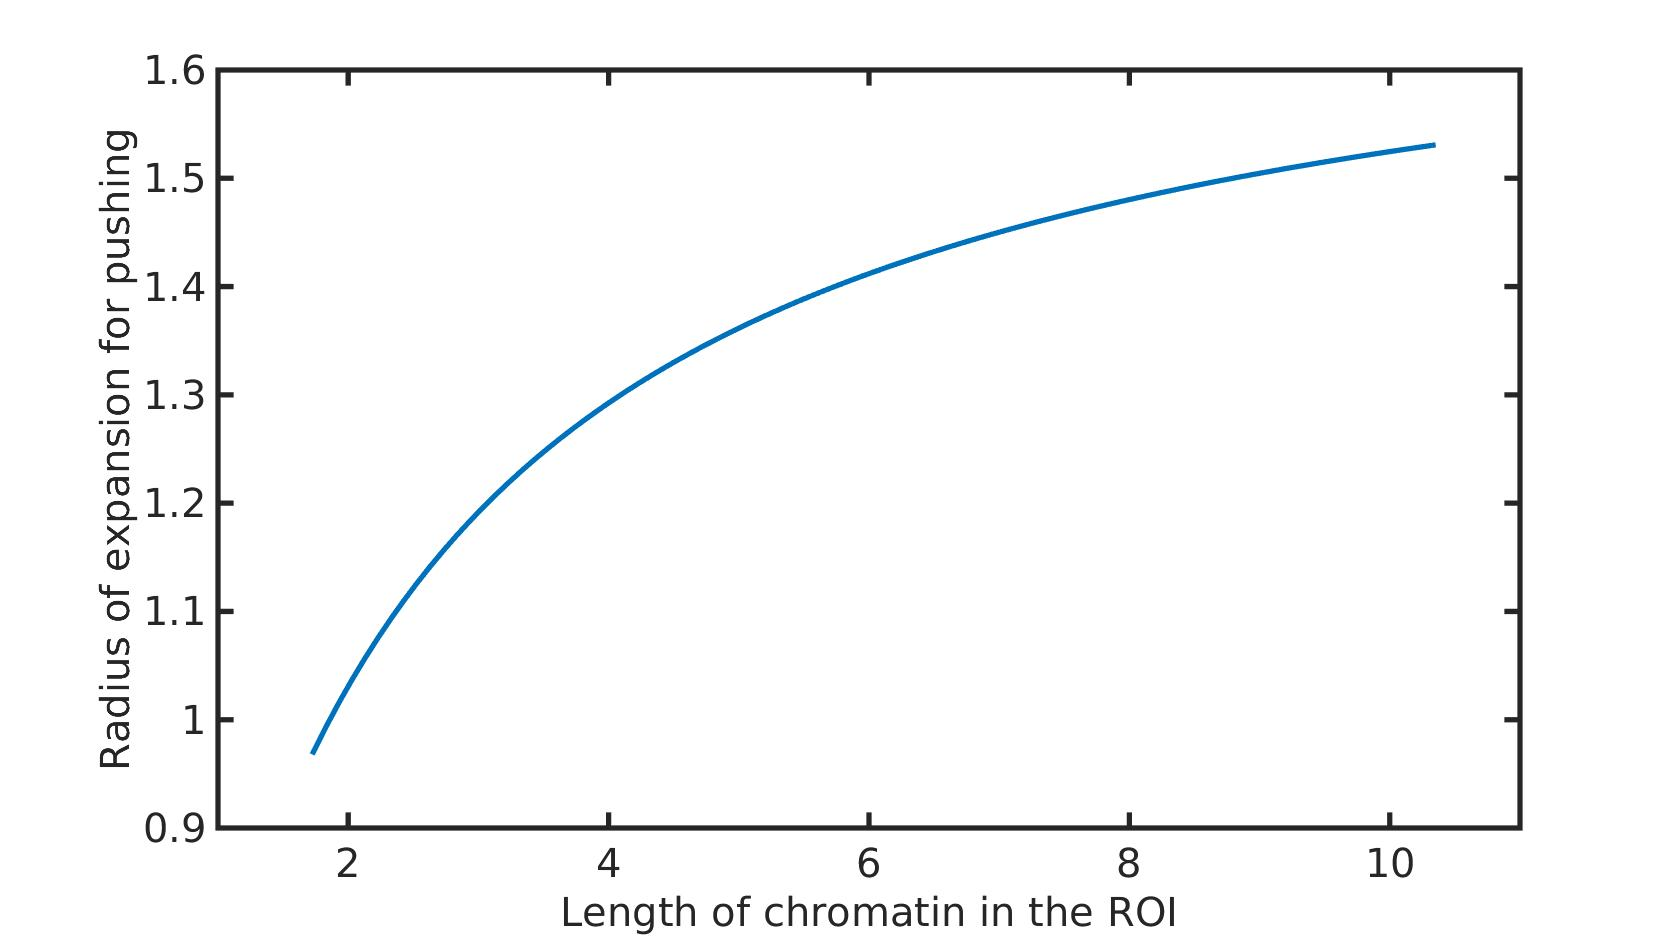
\includegraphics[width=0.5\linewidth, height=0.3\textheight]{Images/SlidingModel/radiusOfPushingVsLengthOfChromainInROI}
			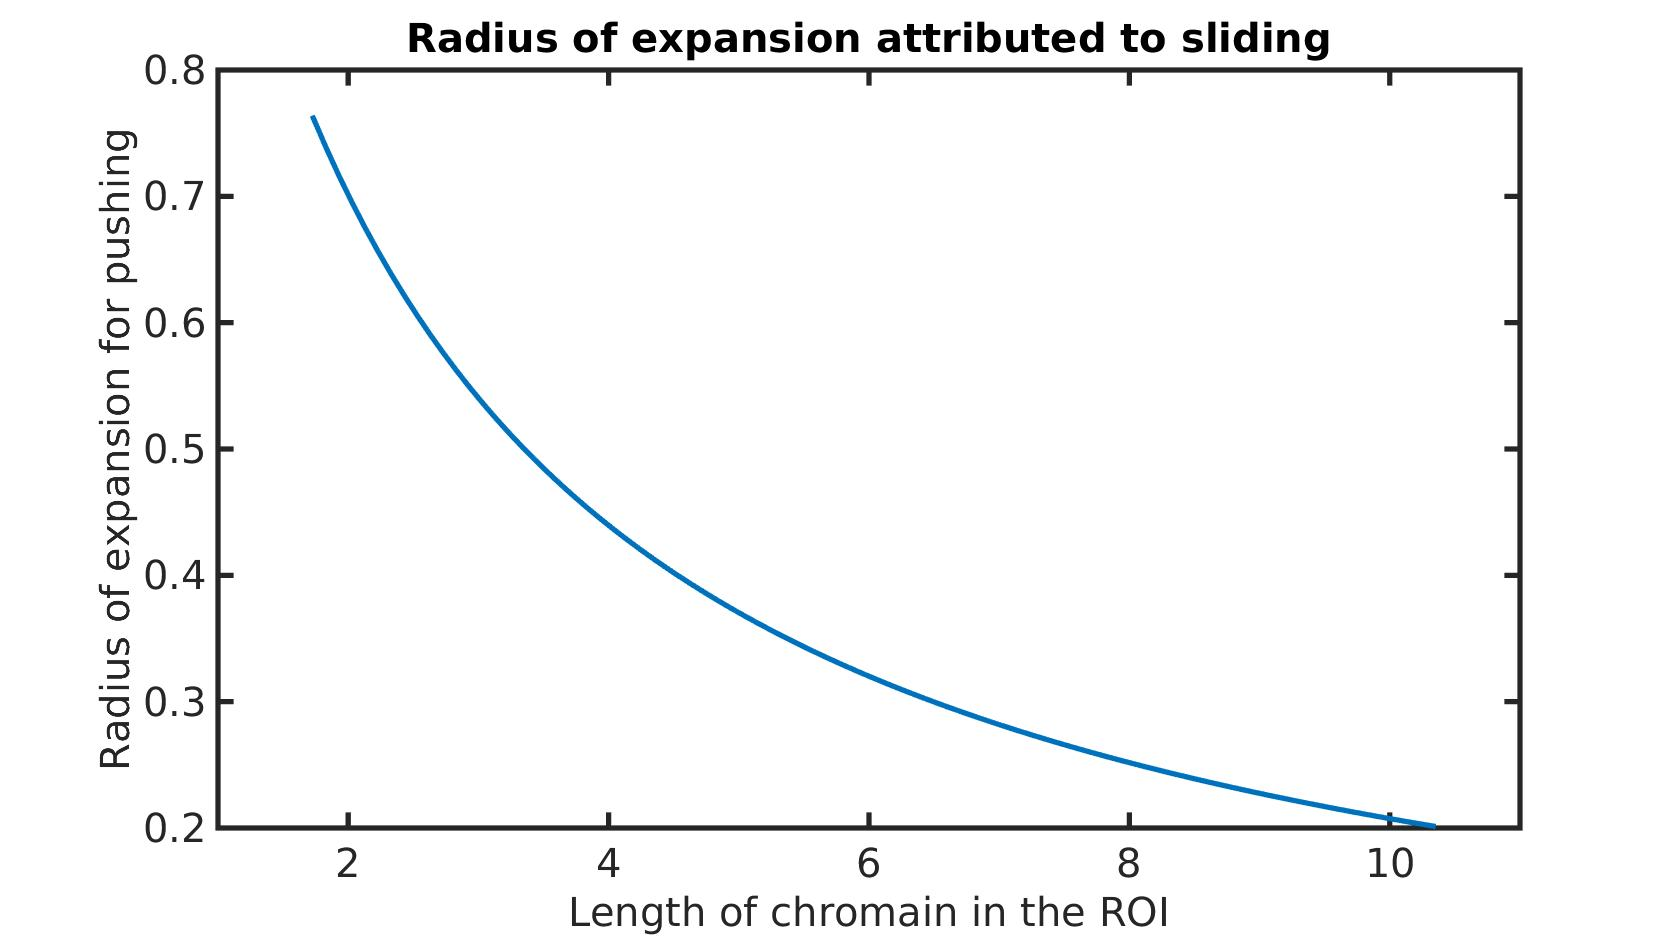
\includegraphics[width=0.5\linewidth, height=0.3\textheight]{Images/SlidingModel/radiusOfSlidingVsLengthOfChromatinInROI}
			\caption{\tiny{The expansion radius attributed to pushing with no sliding (left) of chromatin as a functio of the length of chromatin in the region, and it's complament, the radius of expansion attributed to pushing + sliding (right) as a function of the length of chromatin in the ROI. The ROI expansion is set to $\sqrt{3}$ and values of the chromatin length rang from $\sqrt{3}$ to $7\sqrt{3}$}}
			\label{fig:radiiVsLengthOfChromainInROI}
		\end{figure}
		
									
		\section{Estimation of the contribution of sliding to the expansion from the data}
		We have no direct access to the parameter $l$- the length of chromatin in the ROI. we estimate it indirectly from mass conservation considerations in the illuminated patch.
		By the procedure we offer, we can indirectly measure around 0.25 e
		
		\section{Simulation of expansion and repair}
		
		
		
\end{document}